%%%%%%%%%%%%%%%%%%%%%%%%%%%%%%%%%%%%%%%%%
% Lachaise Assignment
% LaTeX Template
% Version 1.0 (26/6/2018)
%
% This template originates from:
% http://www.LaTeXTemplates.com
%
% Authors:
% Marion Lachaise & François Févotte
% Vel (vel@LaTeXTemplates.com)
%
% License:
% CC BY-NC-SA 3.0 (http://creativecommons.org/licenses/by-nc-sa/3.0/)
%
%%%%%%%%%%%%%%%%%%%%%%%%%%%%%%%%%%%%%%%%%

%----------------------------------------------------------------------------------------
%	PACKAGES AND OTHER DOCUMENT CONFIGURATIONS
%----------------------------------------------------------------------------------------

\documentclass{article}

%%%%%%%%%%%%%%%%%%%%%%%%%%%%%%%%%%%%%%%%%
% Lachaise Assignment
% Structure Specification File
% Version 1.0 (26/6/2018)
%
% This template originates from:
% http://www.LaTeXTemplates.com
%
% Authors:
% Marion Lachaise & François Févotte
% Vel (vel@LaTeXTemplates.com)
%
% License:
% CC BY-NC-SA 3.0 (http://creativecommons.org/licenses/by-nc-sa/3.0/)
% 
%%%%%%%%%%%%%%%%%%%%%%%%%%%%%%%%%%%%%%%%%

%----------------------------------------------------------------------------------------
%	PACKAGES AND OTHER DOCUMENT CONFIGURATIONS
%----------------------------------------------------------------------------------------

\usepackage{amsmath,amsfonts,stmaryrd,amssymb} % Math packages

\usepackage{enumerate} % Custom item numbers for enumerations

\usepackage[ruled]{algorithm2e} % Algorithms

\usepackage[framemethod=tikz]{mdframed} % Allows defining custom boxed/framed environments

\usepackage{graphicx} % images

\usepackage{hyperref}
\graphicspath{ {../outputs/} }

\usepackage{listings} % File listings, with syntax highlighting
\lstset{
	basicstyle=\ttfamily, % Typeset listings in monospace font
}

%----------------------------------------------------------------------------------------
%	DOCUMENT MARGINS
%----------------------------------------------------------------------------------------

\usepackage{geometry} % Required for adjusting page dimensions and margins

\geometry{
	paper=a4paper, % Paper size, change to letterpaper for US letter size
	top=2.5cm, % Top margin
	bottom=3cm, % Bottom margin
	left=2.5cm, % Left margin
	right=2.5cm, % Right margin
	headheight=14pt, % Header height
	footskip=1.5cm, % Space from the bottom margin to the baseline of the footer
	headsep=1.2cm, % Space from the top margin to the baseline of the header
	%showframe, % Uncomment to show how the type block is set on the page
}

%----------------------------------------------------------------------------------------
%	FONTS
%----------------------------------------------------------------------------------------

\usepackage[utf8]{inputenc} % Required for inputting international characters
\usepackage[T1]{fontenc} % Output font encoding for international characters

\usepackage{XCharter} % Use the XCharter fonts

%----------------------------------------------------------------------------------------
%	COMMAND LINE ENVIRONMENT
%----------------------------------------------------------------------------------------

% Usage:
% \begin{commandline}
%	\begin{verbatim}
%		$ ls
%		
%		Applications	Desktop	...
%	\end{verbatim}
% \end{commandline}

\mdfdefinestyle{commandline}{
	leftmargin=10pt,
	rightmargin=10pt,
	innerleftmargin=15pt,
	middlelinecolor=black!50!white,
	middlelinewidth=2pt,
	frametitlerule=false,
	backgroundcolor=black!5!white,
	frametitle={Command Line},
	frametitlefont={\normalfont\sffamily\color{white}\hspace{-1em}},
	frametitlebackgroundcolor=black!50!white,
	nobreak,
}

% Define a custom environment for command-line snapshots
\newenvironment{commandline}{
	\medskip
	\begin{mdframed}[style=commandline]
}{
	\end{mdframed}
	\medskip
}

%----------------------------------------------------------------------------------------
%	FILE CONTENTS ENVIRONMENT
%----------------------------------------------------------------------------------------

% Usage:
% \begin{file}[optional filename, defaults to "File"]
%	File contents, for example, with a listings environment
% \end{file}

\mdfdefinestyle{file}{
	innertopmargin=1.6\baselineskip,
	innerbottommargin=0.8\baselineskip,
	topline=false, bottomline=false,
	leftline=false, rightline=false,
	leftmargin=2cm,
	rightmargin=2cm,
	singleextra={%
		\draw[fill=black!10!white](P)++(0,-1.2em)rectangle(P-|O);
		\node[anchor=north west]
		at(P-|O){\ttfamily\mdfilename};
		%
		\def\l{3em}
		\draw(O-|P)++(-\l,0)--++(\l,\l)--(P)--(P-|O)--(O)--cycle;
		\draw(O-|P)++(-\l,0)--++(0,\l)--++(\l,0);
	},
	nobreak,
}

% Define a custom environment for file contents
\newenvironment{file}[1][File]{ % Set the default filename to "File"
	\medskip
	\newcommand{\mdfilename}{#1}
	\begin{mdframed}[style=file]
}{
	\end{mdframed}
	\medskip
}

%----------------------------------------------------------------------------------------
%	NUMBERED QUESTIONS ENVIRONMENT
%----------------------------------------------------------------------------------------

% Usage:
% \begin{question}[optional title]
%	Question contents
% \end{question}

\mdfdefinestyle{question}{
	innertopmargin=1.2\baselineskip,
	innerbottommargin=0.8\baselineskip,
	roundcorner=5pt,
	nobreak,
	singleextra={%
		\draw(P-|O)node[xshift=1em,anchor=west,fill=white,draw,rounded corners=5pt]{%
		Question \theQuestion\questionTitle};
	},
}

\newcounter{Question} % Stores the current question number that gets iterated with each new question

% Define a custom environment for numbered questions
\newenvironment{question}[1][\unskip]{
	\bigskip
	\stepcounter{Question}
	\newcommand{\questionTitle}{~#1}
	\begin{mdframed}[style=question]
}{
	\end{mdframed}
	\medskip
}

%----------------------------------------------------------------------------------------
%	WARNING TEXT ENVIRONMENT
%----------------------------------------------------------------------------------------

% Usage:
% \begin{warn}[optional title, defaults to "Warning:"]
%	Contents
% \end{warn}

\mdfdefinestyle{warning}{
	topline=false, bottomline=false,
	leftline=false, rightline=false,
	nobreak,
	singleextra={%
		\draw(P-|O)++(-0.5em,0)node(tmp1){};
		\draw(P-|O)++(0.5em,0)node(tmp2){};
		\fill[black,rotate around={45:(P-|O)}](tmp1)rectangle(tmp2);
		\node at(P-|O){\color{white}\scriptsize\bf !};
		\draw[very thick](P-|O)++(0,-1em)--(O);%--(O-|P);
	}
}

% Define a custom environment for warning text
\newenvironment{warn}[1][Warning:]{ % Set the default warning to "Warning:"
	\medskip
	\begin{mdframed}[style=warning]
		\noindent{\textbf{#1}}
}{
	\end{mdframed}
}

%----------------------------------------------------------------------------------------
%	INFORMATION ENVIRONMENT
%----------------------------------------------------------------------------------------

% Usage:
% \begin{info}[optional title, defaults to "Info:"]
% 	contents
% 	\end{info}

\mdfdefinestyle{info}{%
	topline=false, bottomline=false,
	leftline=false, rightline=false,
	nobreak,
	singleextra={%
		\fill[black](P-|O)circle[radius=0.4em];
		\node at(P-|O){\color{white}\scriptsize\bf i};
		\draw[very thick](P-|O)++(0,-0.8em)--(O);%--(O-|P);
	}
}

% Define a custom environment for information
\newenvironment{info}[1][Info:]{ % Set the default title to "Info:"
	\medskip
	\begin{mdframed}[style=info]
		\noindent{\textbf{#1}}
}{
	\end{mdframed}
}
 % Include the file specifying the document structure and custom commands

%----------------------------------------------------------------------------------------
%	ASSIGNMENT INFORMATION
%----------------------------------------------------------------------------------------

\title{COMP9417: Machine Learning Project} % Title of the assignment

\author{z5113817} % Author name and email address

\date{University of New South Wales --- \today} % University, school and/or department name(s) and a date

\newcommand{\injurydef}{a physical injury that leaves a player on the injury list for more than 34 days}
%----------------------------------------------------------------------------------------

\begin{document}

\maketitle % Print the title

%----------------------------------------------------------------------------------------
%	Main Contents
%----------------------------------------------------------------------------------------

% TODO: All code for this project is available \href{https://github.com/william-coulter/NBA-Injury-Predictor}{here}.

\section*{Motivation}

In the 1984 NBA draft, Sam Bowie was drafted as the number 2 pick to the Trail Blazers.
It might be shocking to hear that Bowie was drafted one place \emph{above} the hall of fame superstar Michael Jordan.
This was because the Trail Blazers needed a new superstar "big man" to replace the Center they lossed the season before.
Bowie had an impressive 76 games with the Trail Blazers until a fracture in his left tibia put him out for the season.
Even though Bowie followed the recommened recovery time, the rest of Bowie's career was undermined by the recurring injury.
In 10 seasons with the NBA, Bowie only appeared in 511 games.\\

The question is, even though injuries in sport are seen as an unforeseeable tragedy, can a
machine learning model be used to eliminate some of the unpredictability and quantify
the likelihood that a player will suffer a major injury in the current season?

\section*{The Goal}

Create a model that assigns a likelihood that a player will \emph{suffer a major injury}
in any given season. Suffering a major injury will be defined \injurydef.

\newpage

% TODO: A background on similar projects / how this project is unique?

\section*{The Data}

\subsection*{Datasets}

The datasets were scraped from various sources such as
\href{https://www.prosportstransactions.com/basketball}{prosporttransactions} and
\href{https://www.basketball-reference.com/}{basketball-refrence}. The scrapers
were sourced from \textbf{elap733}'s repository found
\href{https://github.com/elap733/NBA-Injuries-Analysis/tree/master/src/d01_scrapes}{here}.\\

The following datasets can be found in the \textbf{data/raw} directory:
\begin{itemize}
    \item \textbf{player\_stats}: Contains every NBA player's basic statistics for a given season.
    \item \textbf{injury\_list}: Contains information on when players were acquired on and relinquished from NBA injury list.
    \item \textbf{missed\_games}: Contains information on games which players missed (not necessarily due to injury).
    \item \textbf{all\_games\_schedule}: The schedule for every NBA team.
\end{itemize}

The data ranges from 2010 to today.

\subsection*{Cleaning}

For the most part, the data contains pretty clean data with no missing entries
or gibberish values. The datasets were last scraped in 2019 however, so I had to
do some additional scraping to obtain the latest data. Luckily, the scrapers
still worked just fine.\\

For cleaning, all that I had to do was append the latest scraped data
with the existing datasets. The cleaned datasets can be viewed at \textbf{data/cleaned}.
The code used to execute this is stored at \textbf{scripts/clean\_data.py}.

\section*{Processing Data}

% This section explains the reasoning and steps take to produce the \textbf{data/processed/physical\_injuries.csv}
% file and what each of the columns mean. The code used to execute this is stored at
% \textbf{scipts/process\_data.py}.

\subsection*{The Injury List}

This section explains the reasoning and steps take to produce the \textbf{data/processed/physical\_injuries\_2010\_2021.csv}
file and what each of the columns mean. The code used to execute this is stored at
\textbf{scipts/process\_injury\_list.py}.\\

The injury list in the NBA isn't quite as the name suggests. Rather than being a list
of players who are currently suffering from physical injury, players who miss games
for other reasons can be placed on this list. Other reasons include:

\begin{itemize}
    \item \textbf{illness}: 413
    \item \textbf{surgery}: 253
    \item \textbf{COVID-19}: 11
    \item \textbf{personal reasons}: 11
\end{itemize}

In addition, the list includes players who are \emph{relinquished} from their team
(put on the injury list) and players who are \emph{acquired} to their team (removed
from the injury list). This means there are essentially 2 entries for
each individual injury. We want to move the date of this second entry to its own column
so that for each injury we know the dates that player was put on and removed from the
injury list.\\

Earlier I defined a "major injury" as \injurydef. I defined it in this way
by looking at the distribution of days spent on the injury list in our dataset.

\begin{center}
    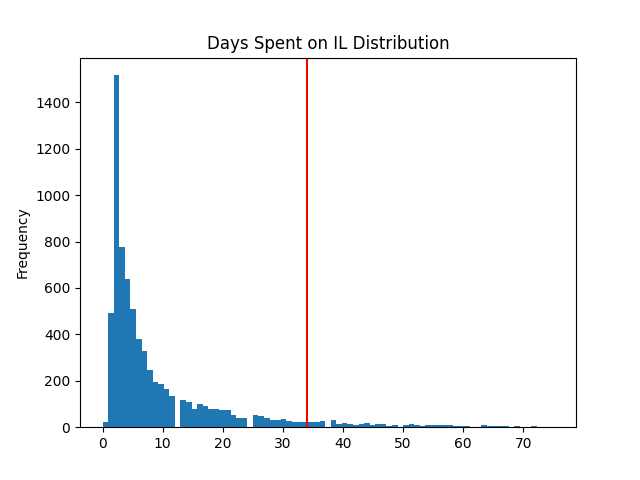
\includegraphics[scale=0.6]{day_spent_on_il_distribution.png}
\end{center}

The red line shows the 80th percentile of this distribution which is at
\textbf{34} days spent on the injury list
\footnote{Some injuries were marked as "player out for season" which means they don't have another entry in the
dataset showing their return. For this case, the player was marked down as being on the IL for 100 days. These players
are not included in the histogram however do play a role in this percentile calculation}.
I selected this to be the boundary between a minor and major. Even though this was done somewhat
arbitarily (I manually decided to use the 80th percentile), I believe this is a
reasonable number since it represents the injuries that left a player on the injury
list for just over a month and represents only 20\% of all NBA injuries since 2010.\\

The processed injury list dataset is stored at \textbf{data/processed/physical\_injuries\_2010\_2021.csv}.
There are \textbf{8,552} entries in this dataset and \textbf{1,711} are major injuries.

\subsection*{Improving the story}

Prior to his career in the NBA, Bowie had developed a stress fracture in his left tibia.
Even though he rested and took the recommended amount of time off for this minor injury,
this would be the same place that Bowie suffered his first major injury when he joined the NBA.\\

Now that we have 1,711 examples where a player were acquired on the injury list
for longer than 34 days, we want to tell a bigger story with these entries by attaching
more data to these injuries. The case of Bowie can inspire us to ask questions such as:

\begin{itemize}
    \item How was the player performing before this injury?
    \item What was their average gametime?
    \item How intense did the player play?
    \item How intense was their team's schedule?
    \item Have they suffered an injury prior?
\end{itemize}

The script \textbf{scripts/derive\_new\_fields.py} attempts to answer some of these questions.\\

The dataset \textbf{data/cleaned/player\_stats\_2010\_2021.csv} contains a general overview of player
statistics for a given season. We can perform a \emph{left join} on this dataset with the processed
physical injuries dataset so that each injury is now linked to the player's performance during
the season that they were injuried.\\
\newpage

\begin{center}
    \begin{table}
    \begin{tabular}{||c c c c c c c c||}
    \hline
    Player & Year & Season & Position & Age & Injury Date & Duration & Notes \\ [0.5ex]
    \hline\hline
    Malik Allen & 2010 & regular & PF & 32 & 2010-10-28 & 9 & placed on IL \\
    \hline
    Malik Allen & 2010 & regular & PF & 32 & 2010-11-10 & 5 & placed on IL \\
    \hline
    Malik Allen & 2010 & regular & PF & 32 & 2010-11-20 & 4 & placed on IL \\
    \hline
    Malik Allen & 2010 & regular & PF & 32 & 2010-11-30 & 1 & placed on IL \\
    \hline
    Malik Allen & 2010 & regular & PF & 32 & 2010-12-23 & 43 & placed on IL with sprained left ankle\\ [1ex]
    \hline
   \end{tabular}
   \caption{\label{tab:multiple-injuries}Dataset showing Malik Allen suffering multiple injuries in the 2010 regular season}
    \end{table}
\end{center}

But what about players who were injured multiple times during the same season? In table \ref{tab:multiple-injuries}, we can see
that Allen suffered a few injuries in the 2010 season. Each of these rows also contain data about
Allen's performance for the 2010 season, which are all identical in their values, since it's all for the
2010 season. Recall that the aim of this model is to predict the likelihood that
a player will suffer a major injury in a given season. Feeding Allen's data into a model
would confuse the model since it has 4 examples where a player didn't suffer a major injury
and 1 example where they did, all with the \emph{exact same} stats for the season.\\

We want to group these examples together so that the model doesn't have contradicting data,
but we also want to keep the information that Allen suffered \emph{minor} injuries
prior to his major injury.\\

Let's create a new field \textbf{Recent Minor Injury Count} which for each
season for a given player, counts the number of minor injuries they received in that season.
A \emph{minor injury} will be defined as an injury that wasn't a major injury.

Let's also create another field \textbf{Previous Major Injury Count} which counts the
number of \emph{major injuries} that a player has suffered strictly prior to that season.
The new dataset is created at \textbf{data/processed/aggregated.csv}.

\subsection*{Tokenising}

Fields such as the player's position and whether the season is post season
or regular are string values. We want to encode these to a numerical value and
store their encoding somewhere.\\

The script \textbf{tokenize\_data.py} performs these operations and stores the
new dataset at \textbf{data/processed/tokenized.csv}.

\subsection*{Normalising and Standardising}

This section explains the steps in \textbf{normalise.py} which is used to
create the dataset at \textbf{date/processed/nomarlised.csv}.

Some players play more minutes per game than others. Because of this, some of fields
such as \emph{FGA} (Field Goal Attempts per game) will be greatly skewed by the
average amount of minutes a player spends in a game. As such, the first step
I have taken to normalise is make all of "per game" stats a ratio with
the average minutes played
\footnote{Note that all normalising and standardising after this point is done \emph{after} training and testing data has been established}.\\

Since the data has a lot of continuous values, it is a good idea to nomralise
these between 0 and 1. I don't want fields such as the age of a player to be weighted significantly
higher than a player's average offensive rebounds per game, just because the value of a player's
age is always much larger.\\

Also, I will assess various models and I do not know the distribution of the dataset
across all of its values. As such, standardising is a good idea.

\subsection*{Data Selection}

I now have a dataset with a lot of meaningful values - almost too many. In the script,
\textbf{select\_data.py} I clean out datapoints that I think will mislead the model (for example, the
player's name) or are correlated and such, provide no further information (for example, Field Goals per game with Field
Goal Attempts per game).
This results in a final processed dataset at \textbf{data/processed/final.csv} which contains the
data that I will be using to train various models on.\\

An explanation on all of the columns contained in this dataset and what they each
mean can be found in appendix \ref{appendix:final-dataset}.

\newpage
\section*{Exploratory Analysis}

I've been doing a bit of exploring of the data previously to
make decisions about deriving new fields for processing.
This section will focus on using the final "processed" dataset
and looking at what we have.

\section*{Model Selection}

\section*{Model Evaluation}

\section*{Conclusion}

\subsection*{Nice to haves}

Would've been nice to incorperate the intensity of the schedule some more.
Do some NLP analysis on the Notes of the injury.

\section*{Appendix}
\label{appendix}

\subsection*{Final Dataset}
\label{appendix:final-dataset}

List of all columns:
\begin{itemize}
    \item \textbf{Season}: whether the row is from regular (1) or post (0) season
\end{itemize}

\end{document}
